\documentclass[a4paper,14pt]{extarticle}

\usepackage[utf8x]{inputenc}
\usepackage[T1,T2A]{fontenc}
\usepackage[russian]{babel}
\usepackage{hyperref}
\usepackage{indentfirst}
\usepackage{here}
\usepackage{array}
\usepackage{graphicx}
\usepackage{caption}
\usepackage{subcaption}
\usepackage{chngcntr}
\usepackage{amsmath}
\usepackage{amssymb}
\usepackage{pgfplots}
\usepackage{pgfplotstable}
\usepackage[left=2cm,right=2cm,top=2cm,bottom=2cm,bindingoffset=0cm]{geometry}
\usepackage{multicol}
\usepackage{askmaps}
\usepackage{titlesec}
\usepackage{listings}
\usepackage{color}
\usepackage{courier}

\definecolor{green}{rgb}{0,0.6,0}
\definecolor{gray}{rgb}{0.5,0.5,0.5}
\definecolor{purple}{rgb}{0.58,0,0.82}

\lstset{
	language=Verilog,
	backgroundcolor=\color{white},   
	basicstyle=\small\ttfamily,
	commentstyle=\color{green},
	keywordstyle=\color{blue},	
	numberstyle=\tiny\color{gray},
	stringstyle=\color{purple},
	breakatwhitespace=false,
	breaklines=true,
	captionpos=b,
	keepspaces=true,
	numbers=left,
	numbersep=5pt,
	showspaces=false,
	showstringspaces=false,
	showtabs=false,
	tabsize=4,
	frame=single,
	inputpath={../quartus/},
	literate={~} {$\sim$}{1}
}

\renewcommand{\le}{\ensuremath{\leqslant}}
\renewcommand{\leq}{\ensuremath{\leqslant}}
\renewcommand{\ge}{\ensuremath{\geqslant}}
\renewcommand{\geq}{\ensuremath{\geqslant}}
\renewcommand{\epsilon}{\ensuremath{\varepsilon}}
\renewcommand{\phi}{\ensuremath{\varphi}}
\renewcommand{\thefigure}{\arabic{figure}} 	
\renewcommand*\not[1]{\overline{#1}}

\titleformat*{\section}{\large\bfseries} 
\titleformat*{\subsection}{\normalsize\bfseries} 
\titleformat*{\subsubsection}{\normalsize\bfseries} 
\titleformat*{\paragraph}{\normalsize\bfseries} 
\titleformat*{\subparagraph}{\normalsize\bfseries} 

\counterwithin{figure}{section}
\counterwithin{equation}{section}
\counterwithin{table}{section}
\newcommand{\sign}[1][5cm]{\makebox[#1]{\hrulefill}}
\graphicspath{{../pics/}}
\captionsetup{justification=centering,margin=1cm}
\def\arraystretch{1.3}
\setlength\parindent{5ex}
\titlelabel{\thetitle.\quad}

\begin{document}

\begin{titlepage}
\begin{center}
	Санкт-Петербургский Политехнический Университет Петра Великого\\[0.3cm]
	Институт компьютерных наук и технологий \\[0.3cm]
	Кафедра компьютерных систем и программных технологий\\[4cm]
	
	\textbf{ОТЧЕТ}\\ 
	\textbf{по лабораторной работе}\\[0.5cm]
	\textbf{SystemVerilog №4}\\[0.1cm]
	Автоматизация проектирования\\ дискретных устройств\\[4.0cm]
\end{center}

\begin{flushright}
	\begin{minipage}{0.45\textwidth}
		\textbf{Работу выполнил студент}\\[3mm]
		группа 33501/4 \hspace*{9mm} Дьячков В.В.\\[5mm]
		\textbf{Преподаватель}\\[5mm]
		\sign[1.5cm] \hspace*{1mm} к.т.н., доц. Филиппов А.С. \\[5mm]
	\end{minipage}
\end{flushright}

\vfill

\begin{center}
	Санкт-Петербург\\
	\the\year
\end{center}
\end{titlepage}

\addtocounter{page}{1}
\counterwithin{lstlisting}{section}

\tableofcontents
\newpage
\listoffigures
\lstlistoflistings
\newpage

\section{lab6\_1}

\subsection{Задание}

На языке Verilog на структурном уровне опишите мультиплексор 2 (4-разрядных входа) $\rightarrow$ 1 (4-разрядный выход), используя мультиплексор \code{mux2_1} 2 (1-разрядных входа) $\rightarrow$ 1 (1-разрядный выход) как компонент структурного описания:
\begin{itemize}
	\item Мультиплексор \code{mux2_1} опишите на структурном уровне с использованием Gate-Level примитивов языка Verilog.
	\item Входы:
		\begin{itemize}
			\item Переключатель \code{sw[3:0]} -- вход \code{ina};
			\item Переключатель \code{sw[7:4]} -- вход \code{inb};
			\item Кнопка \code{pba} – вход управления мультиплексором (кнопка нажата – на выход передается значение с входа \code{ina}, кнопка не нажата -- \code{inb}).
		\end{itemize}
	\item Выходы: светодиоды \code{led[3:0]} – выходы мультиплексора.
\end{itemize}
Дополнительные требования:
\begin{itemize}
	\item[$\circ$] Стандарты и номера выводов СБИС для платы miniDiLaB\_CIV задать с помощью атрибутов.
	\item[$\circ$] Отдельно осуществить моделирование компонента \code{mux2_1} и модуля верхнего уровня иерархии.
\end{itemize}
В описании можно использовать Gate-Level примитивы языка Verilog и созданные компоненты.

\newpage

\subsection{Код на языке Verilog}

В листинге \ref{code:1} приведен код программы на языке Verilog.

\lstinputlisting[caption=lab6\_1.v, label=code:1]{lab6_1/lab6_1.v}

\newpage

\subsection{Результаты синтеза}

На рис. \ref{fig:lab6_1_rtl} приведено изображение синтезированной схемы в RLT Viewer.

\begin{figure}[H]
\begin{center}
	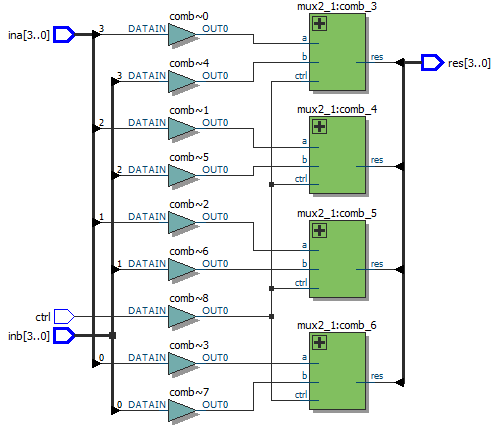
\includegraphics[width=0.7\textwidth]{lab6_1_rtl}
	\caption{Результат синтеза в RLT Viewer}
	\label{fig:lab6_1_rtl}
\end{center}
\end{figure}

\subsection{Результаты моделирования}
\label{sec:lab6_1_modeling}

На рис. \ref{fig:lab6_1_modeling} изображена временная диаграмма работы синтезированного устройства. На вход подаются случайные значения \code{ina[3:0]} и \code{inb[3:0]} сначала при \code{ctrl = 0}, а затем при \code{ctrl = 1}.
\vspace{-0.2cm}
\begin{figure}[H]
\begin{center}
	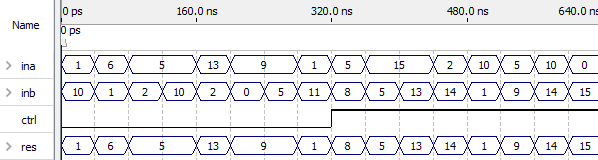
\includegraphics[width=\textwidth]{lab6_1_modeling}
	\caption{Результаты моделирования}
	\label{fig:lab6_1_modeling}
\end{center}
\end{figure}

\subsection{Назначение выводов СБИС}

На рис. \ref{fig:lab6_1_pins} приведены назначения выводов СБИС в Pin Planner.

\begin{figure}[H]
\begin{center}
	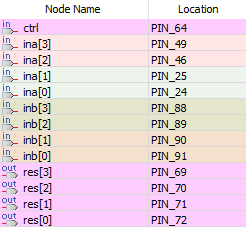
\includegraphics{lab6_1_pins}
	\caption{Таблица назначений в Pin Planer}
	\label{fig:lab6_1_pins}
\end{center}
\end{figure}

\subsection{Результаты проверки на плате}

Для тестирования проекта на плате были использованы тесты, описанные в пункте \ref{sec:lab6_1_modeling}. Результаты тестирования совпадают с ожидаемыми, следовательно, устройство работает верно.

\subsection{Выводы}

Реализовано описание мультиплексора  $2 \rightarrow 1$, используя мультиплексор \code{mux2_1} как компонент структурного описания. Результаты моделирования и тестирования на плате показали, что разработанное устройство работает верно.

\newpage

\section{lab6\_2}

\subsection{Задание}


На основе 8-разрядного последовательного умножителя, осуществляющего умножение младшими разрядами вперед со сдвигом множимого, создайте на языке Verilog параметризированное описание N-разрядного последовательного умножителя, осуществляющего умножение младшими разрядами вперед со сдвигом множимого, в котором:
\begin{itemize}
	\item Параметр \code{N} -- разрядность входных данных (по умолчанию задайте его равным \code{8}) -- операндов.
	\item Параметр \code{INV} --  инверсия выходных данных умножителя ($=1$ выходные данные инвертируются; $=0$ выходные данные не инвертируются).
	\item Загрузка в умножитель новых значений операндов и запуск процедуры умножения должны происходить при изменении любого из операндов:
		\begin{itemize}
			\item При изменении любого из операндов должен формироваться логический аналог сигнала \code{load}, приведенного в примере;
			\item Подсказка: для каждого операнда потребуется регистр для хранения предыдущего значения операнда, которое будет сравниваться с текущим значением операнда.		
		\end{itemize}
	\item Входы (для значения параметра N=4):
		\begin{itemize}
			\item Переключатель \code{sw[7:4]} -- операнд В -- множимое;
			\item Переключатель \code{sw[3:0]} -- операнд А -- множитель.
		\end{itemize}
	\item Выходы: светодиоды \code{led[7:0]} -- выходы умножителя.
\end{itemize}

Дополнительные требования:
\begin{itemize}
	\item[$\circ$] Стандарты и номера выводов СБИС для платы miniDiLaB\_CIV задать с помощью атрибутов.
	\item[$\circ$] Осуществите функциональное моделирование (и приведите в отчете результаты) при: \code{N = 8; INV = 0}.
	\item[$\circ$] Проверку на плате осуществите при: \code{N = 4; INV = 1}.
\end{itemize}
В описании можно использовать любые операторы.

\newpage

\subsection{Код на языке Verilog}

В листинге \ref{code:2} приведен код программы на языке Verilog.

\lstinputlisting[caption=lab6\_2.v, label=code:2]{lab6_2/lab6_2.v}
\vspace{-0.5cm}

\newpage

\subsection{Результаты синтеза}

На рис. \ref{fig:lab6_2_rtl} приведено изображение синтезированной схемы в RLT Viewer при \code{N = 2; INV = 0}.

\begin{figure}[H]
\begin{center}
	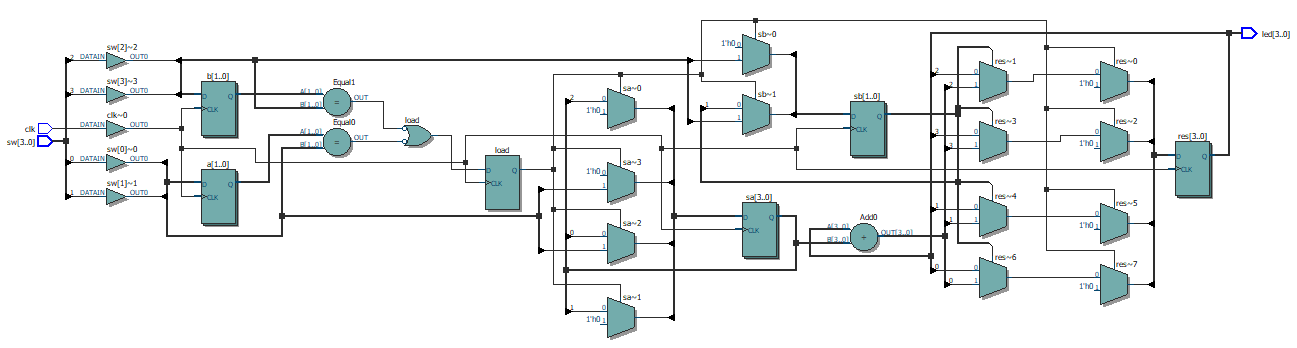
\includegraphics[width=\textwidth]{lab6_2_rtl}
	\caption{Результат синтеза в RLT Viewer}
	\label{fig:lab6_2_rtl}
\end{center}
\end{figure}

\subsection{Результаты моделирования}
\label{sec:lab6_2_modeling}

На рис. \ref{fig:lab6_2_modeling} изображена временная диаграмма работы синтезированного устройства при \code{N = 8; INV = 0}. На вход подаются случайные значения множимого \code{inb[7:0]} и множителя \code{ina[7:0]}, а результат записывается в \code{led[15:0]}.
\begin{figure}[H]
\begin{center}
	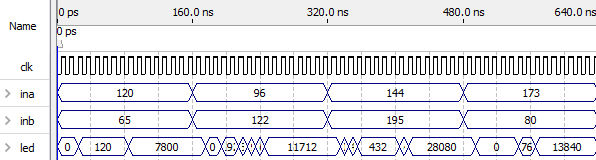
\includegraphics[width=\textwidth]{lab6_2_modeling}
	\caption{Результаты моделирования}
	\label{fig:lab6_2_modeling}
\end{center}
\end{figure}

\newpage

\subsection{Назначение выводов СБИС}

На рис. \ref{fig:lab6_2_pins} приведены назначения выводов СБИС в Pin Planner.

\begin{figure}[H]
\begin{center}
	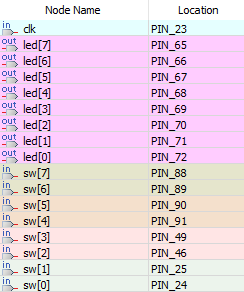
\includegraphics{lab6_2_pins}
	\caption{Таблица назначений в Pin Planer}
	\label{fig:lab6_2_pins}
\end{center}
\end{figure}

\subsection{Результаты проверки на плате}

Для тестирования проекта на плате были использованы тесты, описанные в пункте \ref{sec:lab6_2_modeling} при параметрах \code{N = 4; INV = 1}. Результаты тестирования совпадают с ожидаемыми, следовательно, устройство работает верно.

\subsection{Выводы}

Реализовано параметризированное описание N-разрядного последовательного умножителя, осуществляющего умножение младшими разрядами вперед со сдвигом множимого. Результаты моделирования и тестирования на плате показали, что разработанное устройство работает верно.

\newpage

\section{elab6\_1}

\subsection{Задание}

На языке Verilog создайте параметризированное описание N-разрядного последовательного умножителя, осуществляющего умножение по алгоритму:
\begin{itemize}
	\item Умножение старшими разрядами вперед со сдвигом суммы.
	\item Параметр \code{N} -- разрядность входных данных (по умолчанию задайте его равным 8) -- операндов.
	\item Параметр \code{INV} -- инверсия выходных данных умножителя ($=1$ выходные данные инвертируются; $=0$ выходные данные не инвертируются).
	\item Загрузка в умножитель новых значений операндов и запуск процедуры умножения должны происходить при изменении любого из операндов:
		\begin{itemize}
			\item При изменении любого из операндов должен формироваться логический аналог сигнала \code{load}, приведенного в примере;
			\item Подсказка: для каждого операнда потребуется регистр для хранения предыдущего значения операнда, которое будет сравниваться с текущим значением операнда.
		\end{itemize}
	\item Входы:
		\begin{itemize}
			\item Переключатель \code{sw[7:4]} -- операнд В -- множимое;
			\item Переключатель \code{sw[3:0]} -- операнд А -- множитель.
		\end{itemize}
	\item Выходы: светодиоды \code{led[7:0]} – выходы умножителя.
\end{itemize}

Дополнительные требования:
\begin{itemize}
	\item[$\circ$] Стандарты и номера выводов СБИС для платы miniDiLaB\_CIV задать с помощью атрибутов.
	\item[$\circ$] Осуществите функциональное моделирование (и приведите в отчете результаты) при: \code{N = 8; INV = 0}.
	\item[$\circ$] Проверку на плате осуществите при: \code{N = 4; INV = 1}.
\end{itemize}
В описании можно использовать любые операторы.

\newpage

\subsection{Код на языке Verilog}

В листинге \ref{code:5} приведен код программы на языке Verilog.

\lstinputlisting[caption=elab6\_1.v, label=code:5]{elab6_1/elab6_1.v}

\subsection{Результаты синтеза}

На рис. \ref{fig:elab6_1_rtl} приведено изображение синтезированной схемы в RLT Viewer при \code{N = 2; INV = 0}.

\begin{figure}[H]
\begin{center}
	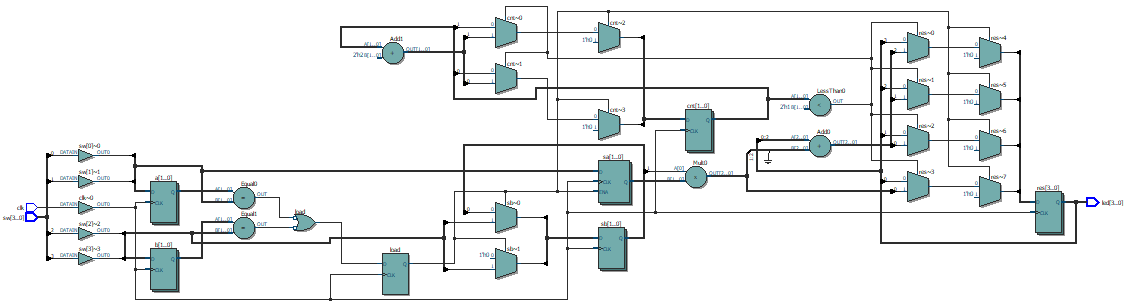
\includegraphics[width=\textwidth]{elab6_1_rtl}
	\caption{Результат синтеза в RLT Viewer}
	\label{fig:elab6_1_rtl}
\end{center}
\end{figure}

\subsection{Результаты моделирования}
\label{sec:elab6_1_modeling}

На рис. \ref{fig:elab6_1_modeling} изображена временная диаграмма работы синтезированного устройства при \code{N = 8; INV = 0}. На вход подаются случайные значения множимого \code{inb[7:0]} и множителя \code{ina[7:0]}, а результат записывается в \code{led[15:0]}.

\begin{figure}[H]
\begin{center}
	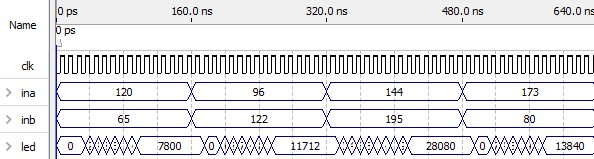
\includegraphics[width=\textwidth]{elab6_1_modeling}
	\caption{Результаты моделирования}
	\label{fig:elab6_1_modeling}
\end{center}
\end{figure}

\newpage

\subsection{Назначение выводов СБИС}

На рис. \ref{fig:elab6_1_pins} приведены назначения выводов СБИС в Pin Planner.

\begin{figure}[H]
\begin{center}
	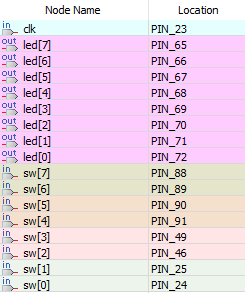
\includegraphics{elab6_1_pins}
	\caption{Таблица назначений в Pin Planer}
	\label{fig:elab6_1_pins}
\end{center}
\end{figure}

\subsection{Результаты проверки на плате}

Для тестирования проекта на плате были использованы тесты, описанные в пункте \ref{sec:elab6_1_modeling} при параметрах \code{N = 4; INV = 1}. Результаты тестирования совпадают с ожидаемыми, следовательно, устройство работает верно.

\subsection{Выводы}

Реализовано параметризированное описание N-разрядного последовательно умножителя, осуществляющего умножение по алгоритму старшими разрядами вперед со сдвигом суммы. Результаты моделирования и тестирования на плате показали, что разработанное устройство работает верно.

\end{document}